In diesem Abschnitt sollen verschiedene Ma{\ss}nahmen gegen Cyber Sickness vorgestellt werden. Dar\"uberhinaus soll erkl\"art werden, warum diese wirkungsvoll sind und was m\"ogliche Nachteile bei der Nutzung entsprechder Ma{\ss}nahmen sein k\"onnten.

Die Ma{\ss}nahmen lassen sich in auf Grund der Sensory Conflict Theory in drei Kategorien einteilen:
Reduktion der Inkongruenz der visuellen Reize entgegen der Erfahrung, indem diese optimiert werden (\autoref{Visuals}), Generation von kongruenten, vestibul\"aren Stimuli entsprechend der Erwartung durch die visuellen Reize (\autoref{Vestibular}) und Adaptation durch den Organismus selbst (\autoref{Adaptation}). Eine generell zu erkennende Tendenz besteht darin, dass diese Methoden versuchen, eine gewohnte \textbf{Nat\"urlichkeit} in der virtuellen Umgebung zu erzeugen.

\subsection{Anpassung der visuellen Reize}\label{Visuals}
Eine Vection passiert dann, wenn ein \textbf{statischer Referenzpunkt} fehlt, an dem man sich optisch fixieren und somit seine Lage relativ dazu sicher feststellen kann. Dies passiert beispielsweise, wenn man aus einem Zug auf einen anderen schaut, ohne den Himmel sehen zu k\"onnen. Wenn der andere Zug sich in Bewegung setzt, erlebt man kurzzeitig Vection, da hier der Himmel als statische Referenz fehlte.

Daher kann ein unabh\"angiger Hintergrund, vorrangig bei CAVE Displays, nach Duh et al.\cite{Duh:2001:Static} helfen. Nat\"urlich ist die Methoden beispielsweise bei Head-Mounted Displays nicht nutzbar, da diese die visuelle Wahrnehmung der tats\"achlichen Umgebung vollst\"andig ersetzen. Eine Methode dennoch einen bekannten Fixpunkt in die virtuelle Umgebung zu integrieren ist die virtuelle Nase wie in \autoref{abb:vnose}, die laut Wienrich et al.\cite{Wienrich:2018:Nose} die Intensit\"at von Cyber Sickness bei Nutzung von Head-Mounted-Displays reduzieren kann.


\begin{figure}[b]
	\centering 
	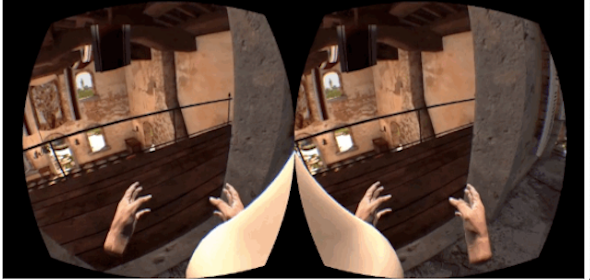
\includegraphics[width=\columnwidth]{virtual_nose.png}
	\caption{Virtuelle Nase zur Reduktion von Cyber Sickness bei Head-Mounted Displays. Bild von WIRED\cite{WIRED:2020:Nose}, letzter Zugriff: 03.05.2020}
	\label{abb:vnose}
\end{figure}


Desweiteren ist es f\"ur die Reduktion von Cyber Sickness ratsam, wenn die graphische Darstellung und Design der virtuellen Umgebung sich dadurch auszeichnen, dass sie nat\"urlich wirken und ruhige, weite Szenen ohne schnellwechselnde Bewegungen nachbildet. Die Parameter der Graphik sollten wie folgt umgesetzt werden:

Die Aufl\"osung und Wiederholungsrate\footnote{50-60 Hz, nach Simon et al.\cite{Simon:2014:Factors}} sollten angemessen hoch sein\cite{kirollos:2019:refresh}, das \textit{Field of View} sollte sich nach Fernandes et al.\cite{Fenandes:2016:FOV} dynamisch anpassen und tendenziell eher klein sein und hoch \"uber dem Boden ansetzen, sofern der Kontext, f\"ur den die virtuelle Umgebung genutzt wird, das zul\"asst. Geringe Latenz f\"uhrte nach Meehan et al.\cite{Meehan:2003:latency} zu mehr wahrgenommener Presence und laut Simon et al.\cite{Simon:2014:Factors} auch zu Cyber Sickness, ebenso wie durch Flickern in der Darstellung der virtuellen Umgebung.
Bei all diesen Punkten stellt sich immer die Frage des Aufwandes und der Umsetzbarkeit durch die verf\"ugbare Hardware.

Es scheint, als verursachen realistischere Graphik bzw. Animationen st\"arkere Cyber Sickness\cite{Pouke:2018:Realism}.
In Anbetracht der beiden Punkte, statische Referenz und Nat\"urlichkeit, empfehlen sich weite Landschaften in virtuellen Umgebungen und im Sinne der Sensory Conflict Theory, Fortbewegung in Virtual Reality m\"oglichst zu reduzieren\footnote{In Computerspielen zum Beispiel Teleportation nutzen}, wobei sich hier erneut das Problem aufwirft, dass diese Methoden nicht in jedem Kontext der Virtual Reality einsetzbar sind.

Obwohl mit den genannten Anpassung der visuellen Komponente die Vection schon wesentlich angenehmer und weniger gest\"ort durch Cyber Sickness sein kann, sodass auch eine Immersion in die virtuelle Umgebung stattfindet, ist es immer m\"oglich zus\"atzlich kongruente, vestibul\"are Stimuli zu erzeugen, sodass die Vection keine Illusion mehr ist, sondern nahe an das tats\"achliche Bewegungserlebnis herankommt.


\subsection{Erzeugen kongruenter Stimuli}\label{Vestibular}

Zu den visuellen Reizen der virtuellen Umgebung k\"onnen die verschiedenen Sinneskan\"ale kongruente Stimuli erg\"anzen, auch durch auditive oder haptische, um die Orientierung im virtuellen Raum zu erh\"ohen. Vorrangig l\"asst sich Cyber Sickness aber reduzieren, indem man eine entsprechende M\"oglichkeit der Bewegung einr\"aumt, w\"ahrend man in der virtuellen Umgebung ist. Dies ist vor allem durch sogenannte VRN-Chairs und Treadmills m\"oglich.

VRN-Chairs sind Rollst\"uhle, die mit magnetischen Sensoren ausgestattet werden, sodass die Bewegung der R\"ader des Rollstuhls passend in die Virtual Reality \"ubertragen werden kann. Durch gleichgerichtete Drehung der R\"ader kann eine Vor- oder R\"uckw\"artsbewegung, durch entgesetzte Drehnung eine Rotation in die jeweilige Richtung erzeugt werden. Durch das unterschiedlich starkes Drehen k\"onnen Kurven gefahren werden. Laut Byagowi\cite{Byagowi:2014:VRNchair} reduzieren VRN-Chairs Cyber Sickness und haben den Vorteil, dass sie barrierefrei sind, sodass sie auch in speziellen medizinischen Szenarien genutzt werden k\"onnen. Generell treten im Sitzen in Virtual Reality weniger Symptome von Cyber Sickness auf. VRN-Chairs haben jedoch Nachteile in virtuellen Umgebung, die die dritte Dimension stark beanspruchen und sind somit nicht in allen Kontexten nutzbar.

Eine weitere M\"oglichkeit der Bewegung w\"ahrend man in der virtuellen Realit\"at ist, sind Treadmills. Diese sind in der Regel omnidirektional, sodass sich frei in alle Richtungen bewegen kann. Nach Aldaba und Moussavi\cite{Aldaba:2019:VRNTread} sind VRN Chairs aber gegen\"uber Treadmills effektiver, da sie den Reizen der nat\"urlichen Bewegung eher entsprechen und dadurch die Symptome der Cyber Sickness weniger intensiv sind wie in \autoref{abb:comp_vrn_tread} zu sehen ist. Desweiteren beantspruchen Treadmills oft viel Raum. Au{\ss}erdem sind sie gegen\"uber VRN-Chairs nicht barrierfrei und wesentlich kostenintensiver.

\begin{figure}[tbh]
	\centering 
	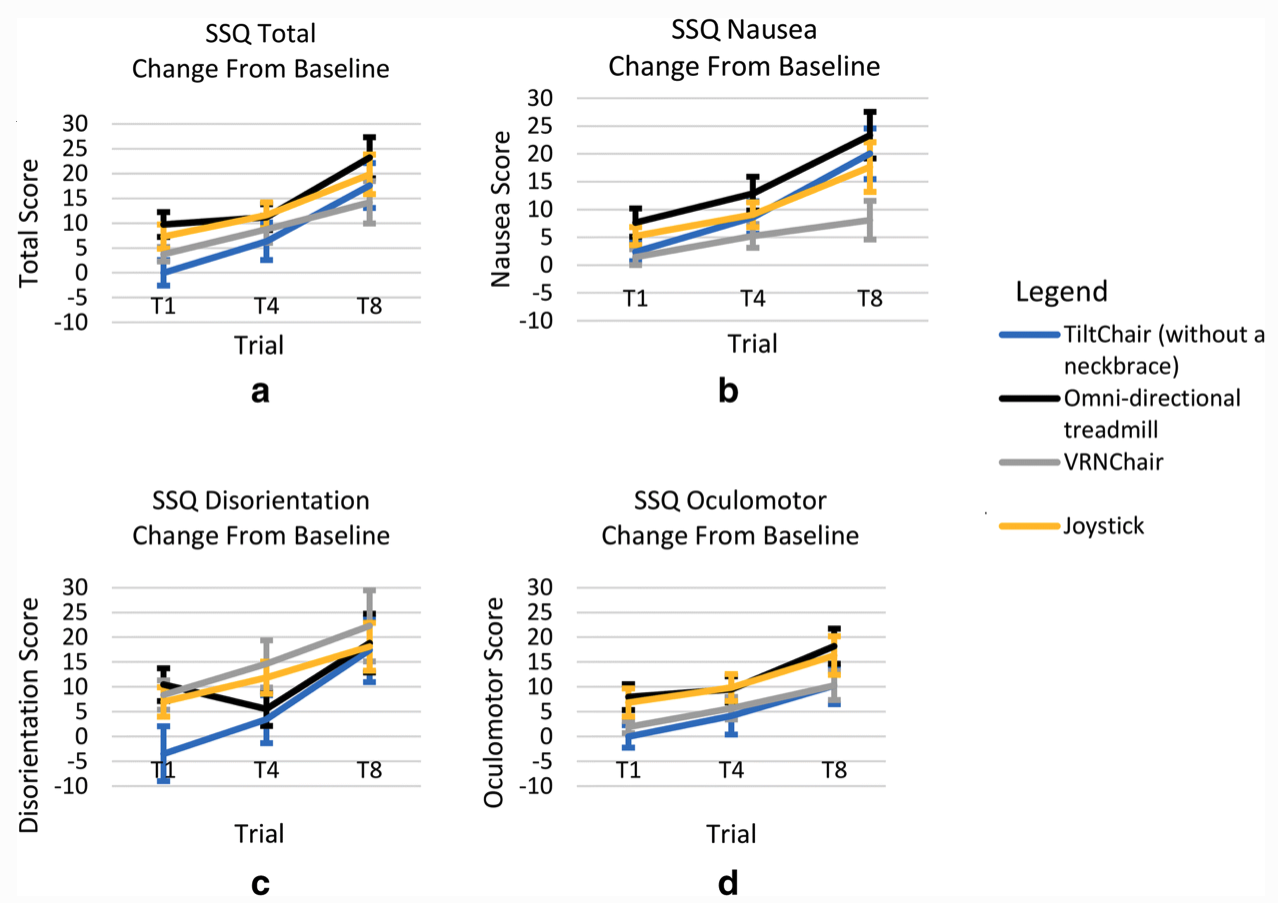
\includegraphics[width=\columnwidth]{comparision_vrn_tread.png}
	\caption{Vergleich verschiederer Methoden bez\"uglich Cyber Sickness von Aldaba und Moussavi\cite{Aldaba:2019:VRNTread}. Niederige SSQ-Scores bedeuten weniger Cyber Sickness.}
	\label{abb:comp_vrn_tread}
\end{figure}

Ohne eine tats\"achlich stattfindende Bewegung, die dann durch die Tr\"agheit der Fl\"ussigkeit in den Bogeng\"angen des Innenohrs einen Reiz erzeugt, funktioniert die \textit{galvanische Vestibul\"arstimulation}, bei der das Gleichgewichtsorgan nicht-invasiv direkt stimuliert wird. Nach Weech et al.\cite{Weech:2020:GVS} kann sie kurzzeitig Cyber Sickness reduzieren, w\"ahrend und kurz nach der Reizung.
Galvanischen Vestibul\"arstimulation scheint effektiv zu sein, weil der Organismus in der virtuellen Umgebung die Gewichtung der Sinneskan\"ale neu bestimmt. Vestibul\"are Reize werden als unzuverl\"assig empfunden und es finden ein \textit{Down-Weighing} statt, wogegen sich mehr auf die visuellen Stimuli verlassen wird und diese st\"arker gewichtet werden.
Der Nachteil der galvanischen Vestibul\"arstimulation ist, dass dieses Verfahren noch relativ unerforscht ist, und bis jetzt nicht bekannt ist, wie es sich auf h\"ohere kognitiven Schichten auswirken kann.

Wenn ein Organismus sich in kurzen Zeitfenstern, schon anzupassen beginnt, stellt sich die Frage, wie die Adaptation auf l\"angere Zeit mit regelm\"a{\ss}iger Nutzung virtueller Realit\"aten aussieht und welche weiteren Faktoren das Auftreten von Cyber Sickness noch beeinflussen k\"onnen.

\subsection{Adaptation und interindividuelle Faktoren}\label{Adaptation}

langfristige Adaptation

Equipement/Passform

Age simon et al.
Gender 
Illness
Posture

Control
Duration Aldaba 
